\documentclass[tikz,border=6pt]{standalone}
\usepackage[T1]{fontenc}\usepackage{newtxtext,newtxmath}\usepackage{tikz}
\usetikzlibrary{arrows.meta,positioning,calc}
\definecolor{ink}{HTML}{172033}\definecolor{greyLine}{HTML}{9CA3AF}
\definecolor{greyFill}{HTML}{F3F4F6}\definecolor{qkC}{HTML}{B91C1C}
\definecolor{ovC}{HTML}{0B7285}\definecolor{steerC}{HTML}{2E7D32}
\tikzset{>={Latex[length=2.4mm,width=1.7mm]},
  ctitle/.style={font=\bfseries,text=ink,align=center},
  rowlab/.style={font=\small\bfseries,align=center},
  poslab/.style={font=\scriptsize\bfseries,text=ink,align=center},
  feat/.style={draw,line width=0.8pt,rounded corners=2pt,minimum width=13mm,
    minimum height=10mm,font=\footnotesize\bfseries,text=ink,inner sep=1pt,align=center},
  alab/.style={font=\scriptsize,text=ink,fill=white,inner sep=0.6pt},
  keytxt/.style={font=\scriptsize,text=ink,align=left,anchor=west}}
\begin{document}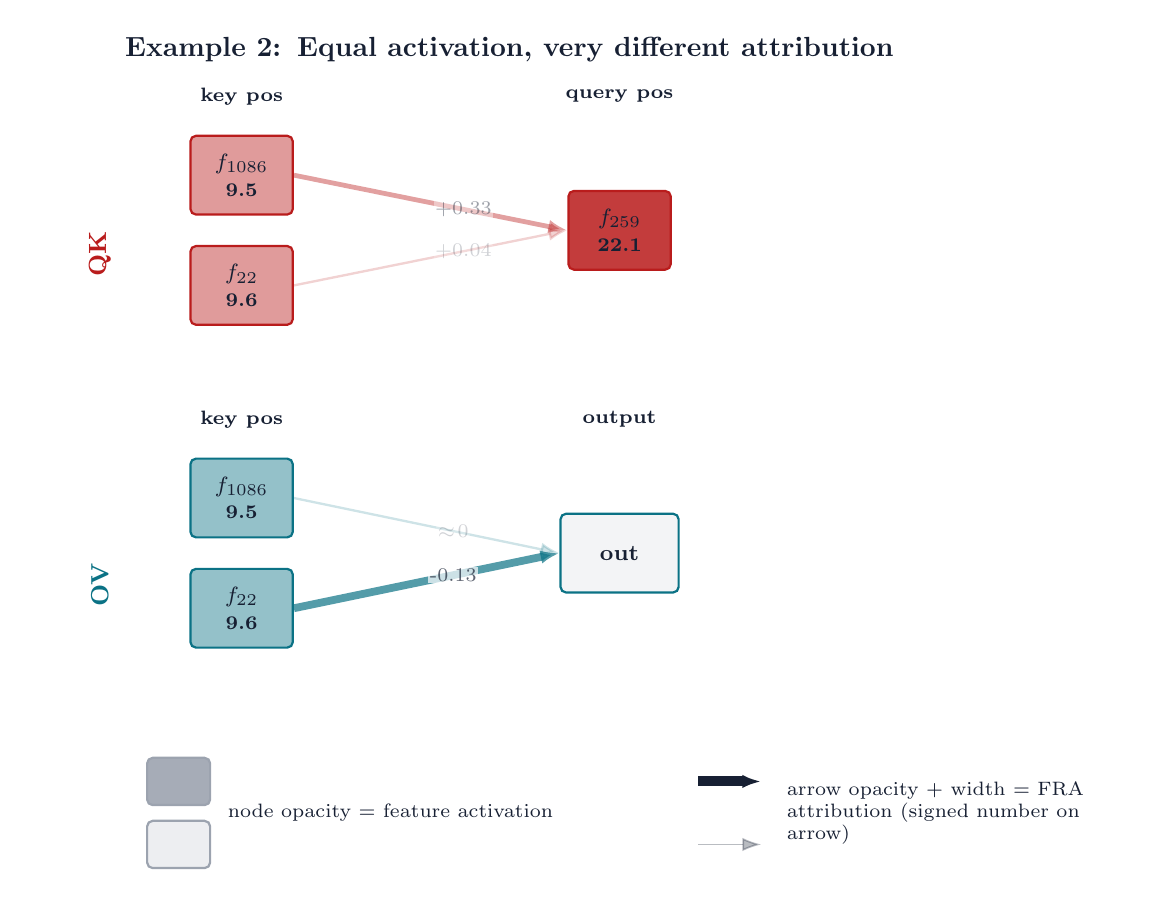
\begin{tikzpicture}[x=1mm,y=1mm]
\node[ctitle,text width=120mm] at (50,96) {Example 2: Equal activation, very different attribution};
\node[rowlab,text=qkC,rotate=90] at (-2,70) {QK};
\node[rowlab,text=ovC,rotate=90] at (-2,28) {OV};
\node[poslab] at (16,90) {key pos};\node[poslab] at (64,90) {query pos};
\node[feat,draw=qkC,fill=qkC!44] (k1086) at (16,80) {$f_{1086}$\\{\scriptsize 9.5}};
\node[feat,draw=qkC,fill=qkC!44] (k22) at (16,66) {$f_{22}$\\{\scriptsize 9.6}};
\node[feat,draw=qkC,fill=qkC!86] (q259) at (64,73) {$f_{259}$\\{\scriptsize 22.1}};
\draw[->,qkC,line width=1.72pt,opacity=0.42] (k1086.east) -- node[alab,pos=0.62]{+0.33} (q259.west);
\draw[->,qkC,line width=0.85pt,opacity=0.20] (k22.east) -- node[alab,pos=0.62]{+0.04} (q259.west);
\node[poslab] at (16,49) {key pos};\node[poslab] at (64,49) {output};
\node[feat,draw=ovC,fill=ovC!44] (o1086) at (16,39) {$f_{1086}$\\{\scriptsize 9.5}};
\node[feat,draw=ovC,fill=ovC!44] (o22) at (16,25) {$f_{22}$\\{\scriptsize 9.6}};
\node[feat,draw=ovC,fill=greyFill,minimum width=15mm] (out) at (64,32) {out};
\draw[->,ovC,line width=0.84pt,opacity=0.20] (o1086.east) -- node[alab,pos=0.60]{$\approx\!0$} (out.west);
\draw[->,ovC,line width=2.81pt,opacity=0.70] (o22.east) -- node[alab,pos=0.60]{-0.13} (out.west);
\node[feat,draw=greyLine,fill=greyLine!90,minimum width=8mm,minimum height=6mm] at (8,3){};
\node[feat,draw=greyLine,fill=greyLine!18,minimum width=8mm,minimum height=6mm] at (8,-5){};
\node[keytxt] at (13,-1) {node opacity $=$ feature activation};
\draw[->,ink,line width=3.6pt] (74,3)--(82,3);\draw[->,ink,line width=0.6pt,opacity=0.3] (74,-5)--(82,-5);
\node[keytxt,text width=42mm] at (84,-1) {arrow opacity $+$ width $=$ FRA attribution (signed number on arrow)};
\end{tikzpicture}\end{document}
